\section{Applications of Huffman Code}

1. JPEG 图像压缩 \\
<1>. 离散余弦变换(Discrete cosine transform DCT). \\
<2>. 量化(Quantization). $z=\text{round}\left(\dfrac{y}{q}\right)$, $q$ 为量化步长. \\
<3>. 对直流分量(DC)应用 DPCM Huffman tree(根据先验的现成的树), 交流分量(AC)用行程码编码. \\

\begin{figure}[htbp]
    \centering
    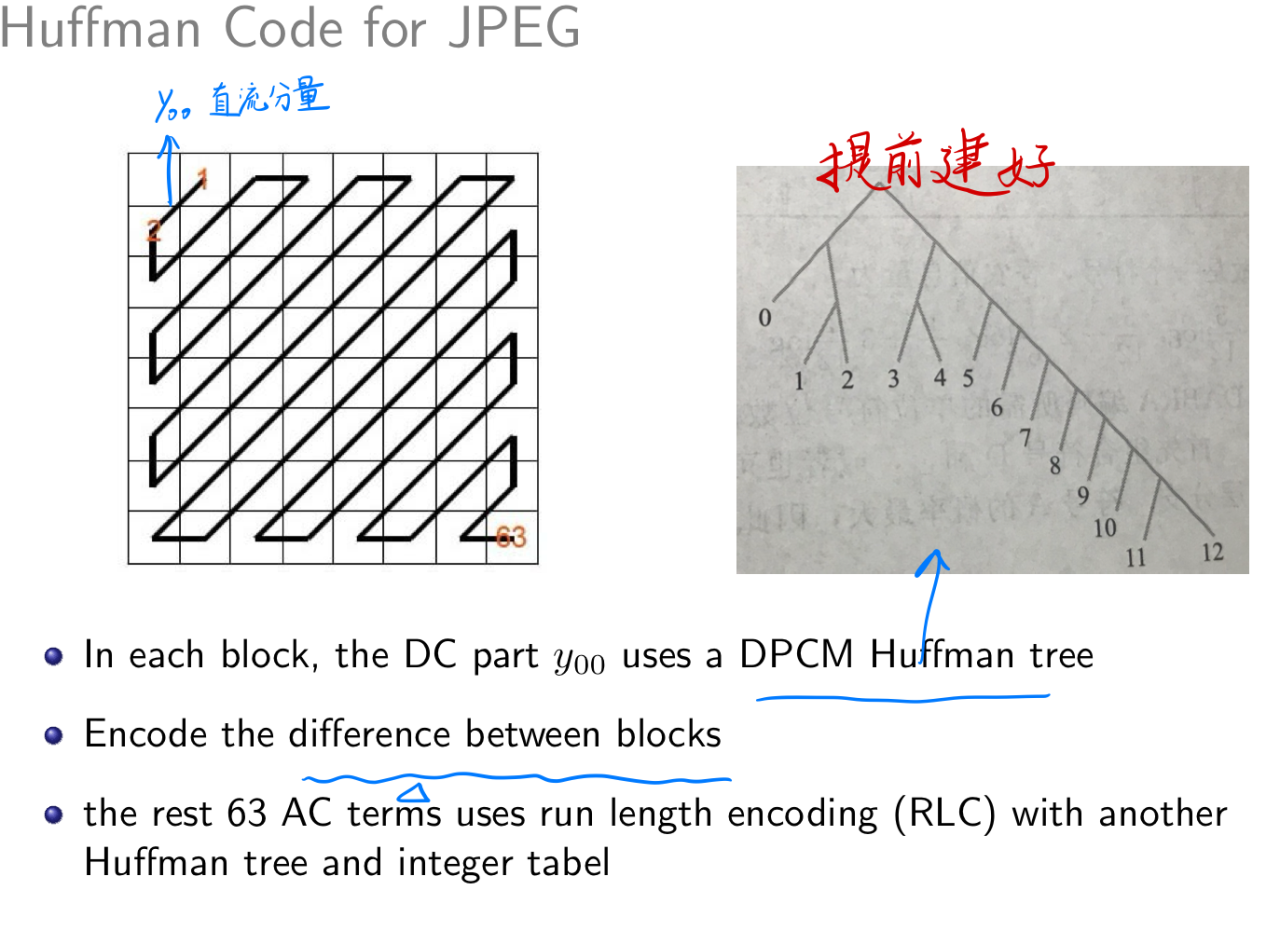
\includegraphics[width=1.1\textwidth]{./figures/chapter3/jpeg1.png}
    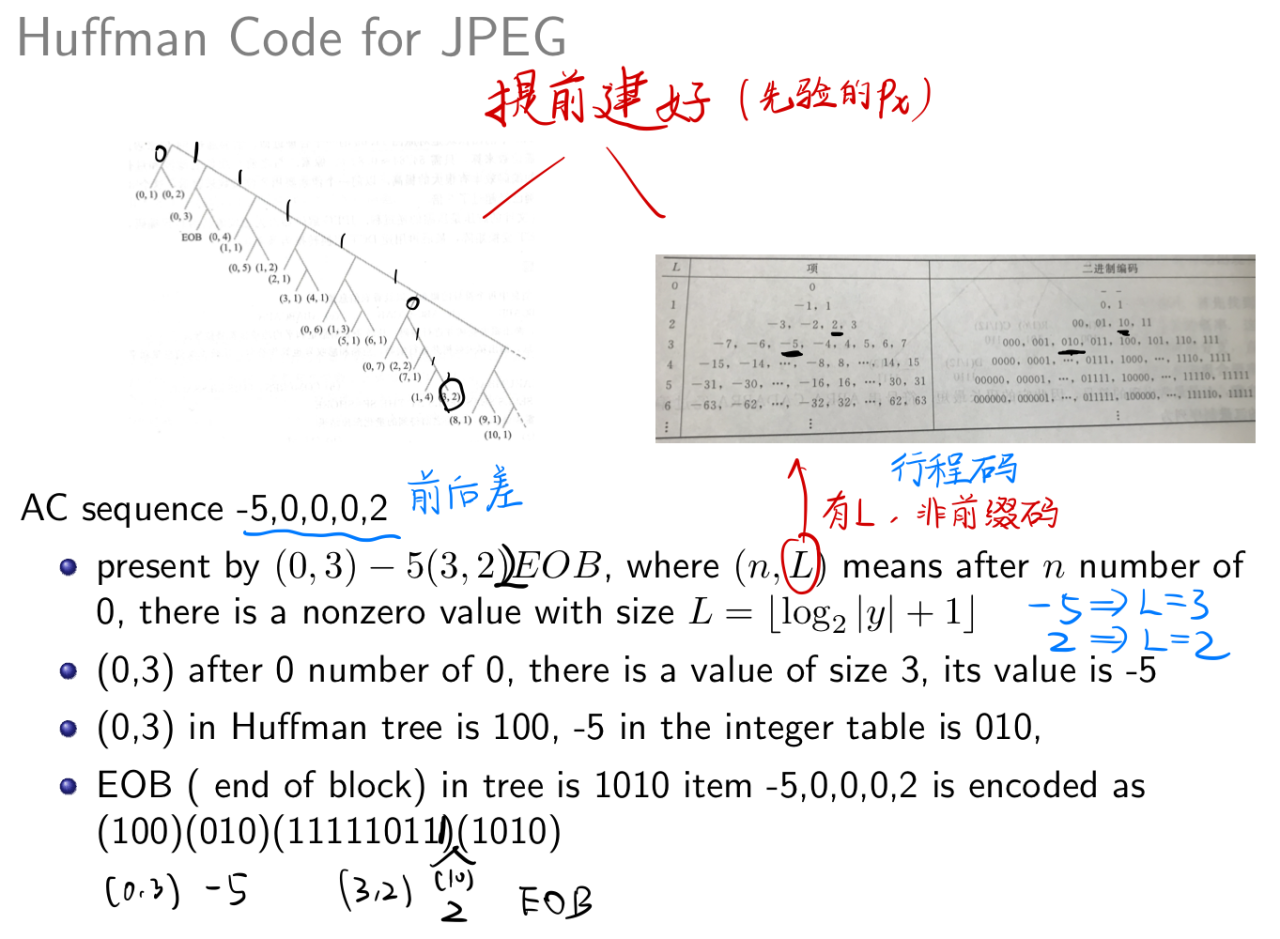
\includegraphics[width=1.1\textwidth]{./figures/chapter3/jpeg2.png}
\end{figure}

\begin{figure}[htbp]
    \centering
    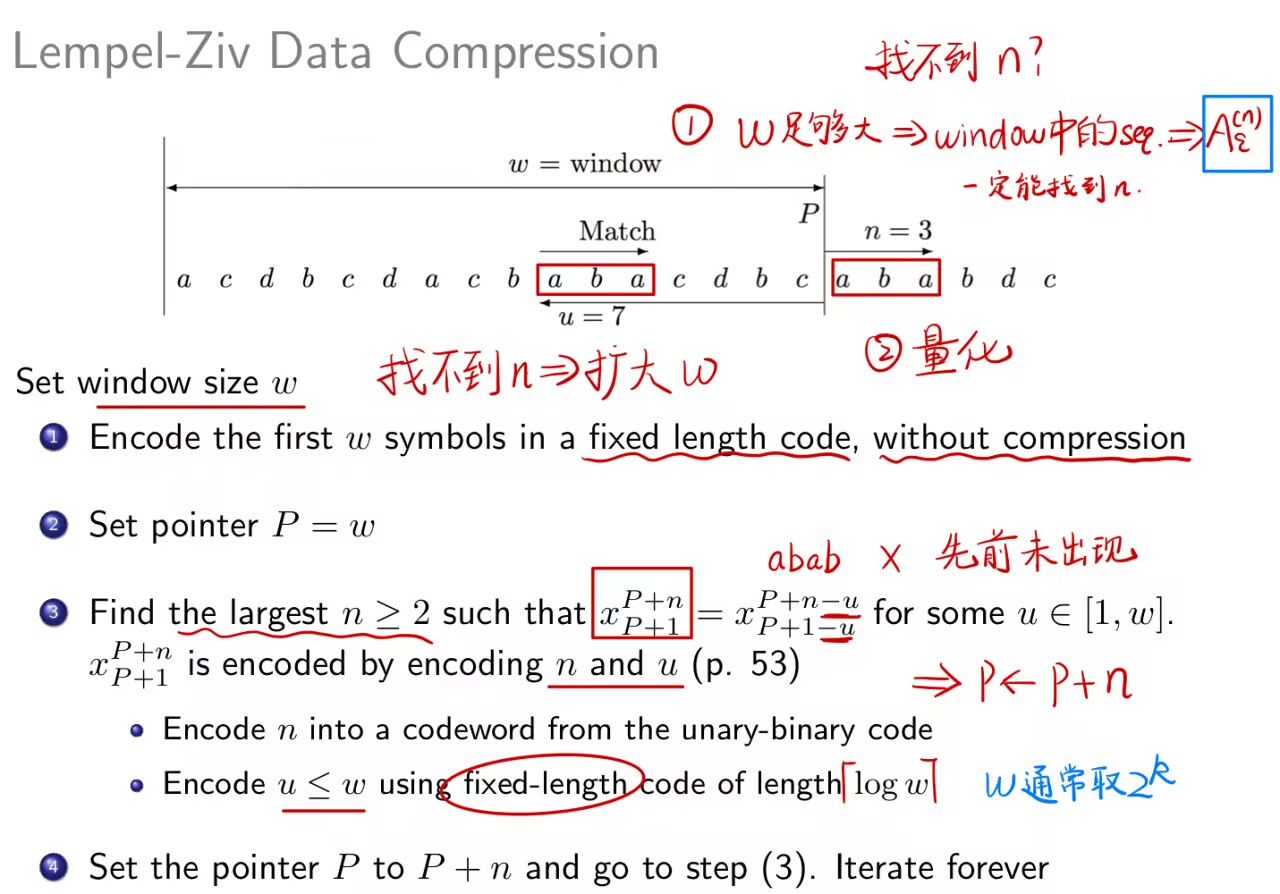
\includegraphics[width=1\textwidth]{./figures/chapter3/lempel_ziv1.png}
    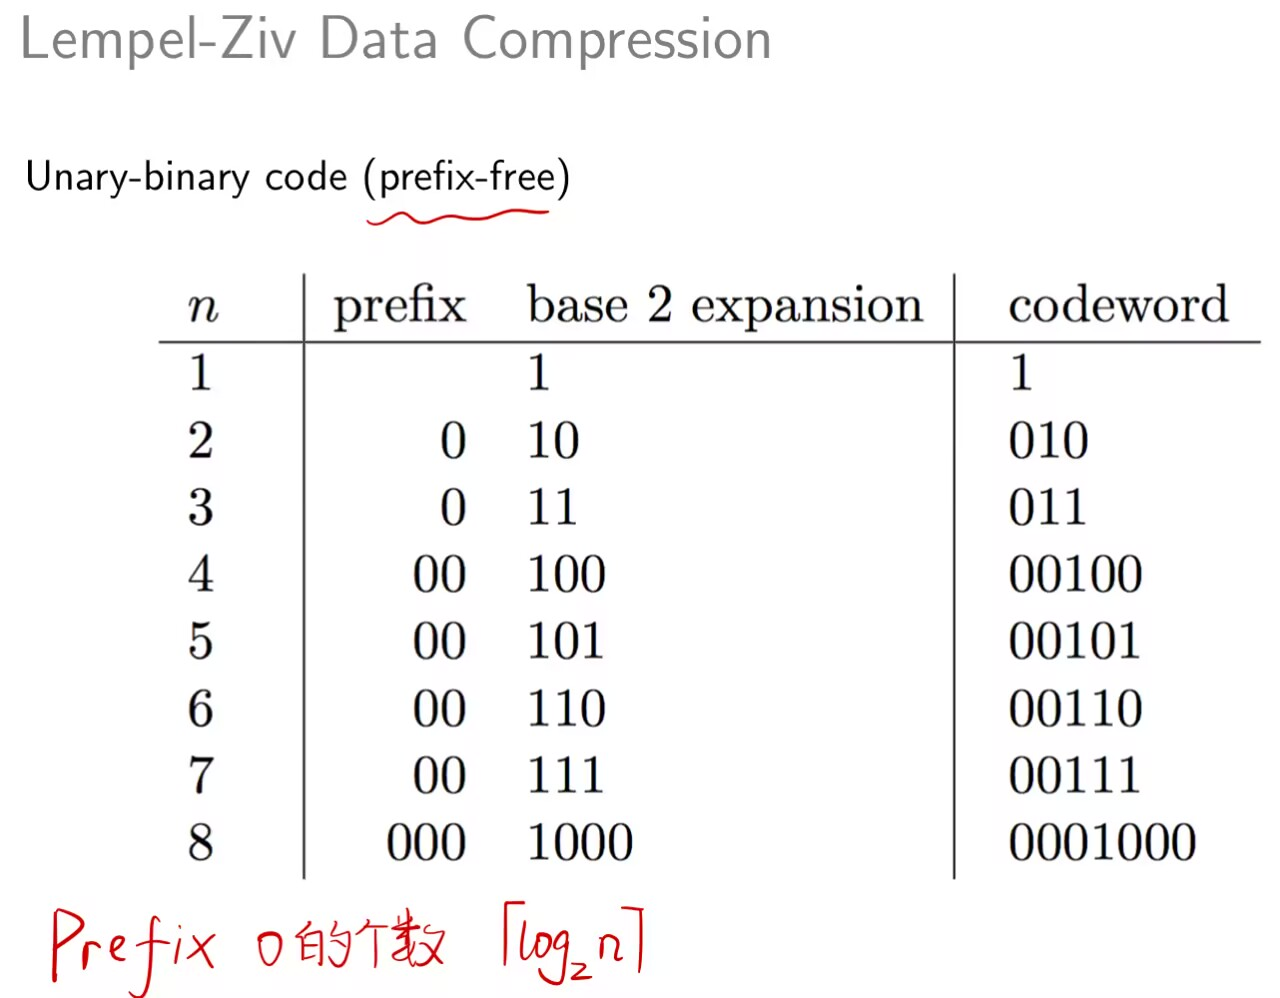
\includegraphics[width=1\textwidth]{./figures/chapter3/lempel_ziv2.png}
\end{figure}
2. Lempel-Ziv Data Compression

Lempel-Ziv 算法的思想是利用历史数据的重复性来估计真实的概率分布$p(x)$, 而不去预测 $q(x)$, 达到自适应最小化.

若数据的真实分布为 $p(x)$, 根据先验得出的概率分布为 $q(x)$, 则使用 $q(x)$ 进行 Huffman coding 与最优解的差距:
\begin{align*}
\Delta &= \sum_{x} p(x) \log \frac{1}{q(x)} - \sum_{x} p(x) \log \frac{1}{p(x)} \\
&= \sum_{x} p(x) \log \frac{p(x)}{q(x)} \\
&= D(p\|q)
\end{align*}

当窗口 $w$ 足够大时, window中的 sequence 可以看作是 typical set: $A_{\epsilon}^{(n)}$, 可以视作 w.p. 1 的可以找得到$n$.

所以引出下一章的内容: Asymptotic Equipartition Property(AEP).